\documentclass{report}

\usepackage{graphicx}
\usepackage{caption}

\newcommand{\source}[1]{\caption*{Source: {#1}} }

\usepackage[
    style=ieee
    ]{biblatex}
\addbibresource{bitcoin-a-peer-to-peer-electronic-cash-system.bib}
\addbibresource{Distributed-Ledger-Technology.bib}
\addbibresource{BaaS-analysis.bib}
\addbibresource{chaincode-performance-analysis.bib}
\addbibresource{A-Privacy-Preserving-Healthcare-Framework-Using-Hyperledger-Fabric.bib}
\addbibresource{Comparison-of-Smart-Contract-Blockchains-for-Healthcare-Applications.bib}
\addbibresource{distributed-systems-concepts-design.bib}
\addbibresource{GDPR.bib}
\addbibresource{On-the-Security-and-Privacy-of-Hyperledger-Fabric-Challenges-and-Open-Issues.bib}
\addbibresource{Penetration-Testing-Technical-Report.bib}
\addbibresource{Research-advances-on-blockchain-as-a-service-architectures-applications-and-challenges.bib}
\addbibresource{the-byzantine-generals-problem.bib}
\addbibresource{Using-Blockchain-for-Electronic-Health-Records.bib}
\addbibresource{Variants-vaccines-and-vaccination-passports-Challenges-and-chances for-travel-medicine.bib}
\addbibresource{Hyperledger_Arch_WG_Paper_1_Consensus.bib}
\addbibresource{Design-and-Implementation-on-Hyperledger-Based-Emission-Trading-System.bib}
\addbibresource{IBM-Blockchain-Platform-Technical-Overview.bib}
\addbibresource{Analysis-and-Design-of-Cryptographic-Hash-Functions-MAC-Algorithms-and-Block-Ciphers.bib}
\addbibresource{secrecy-authentication-and-public-key-systems.bib}
\addbibresource{Implementation-Considerations-for-Blockchain-in-Healthcare-Institutions.bib}
\addbibresource{Whats-new-in-Hyperledger-Fabric-v2.bib}
\addbibresource{Hyperledger-Fabric-A-Distributed-Operating-System-for-Permissioned-Blockchains.bib}
\addbibresource{ETHEREUM-A-SECURE-DECENTRALISED-GENERALISED-TRANSACTION-LEDGER.bib}
\addbibresource{Implementing-fault-tolerant-services-using-the-state-machine-approach-a-tutorial.bib}
\addbibresource{ethereum-whitepaper.bib}
\addbibresource{Decentralized-Consensus-for-Edge-Centric-Internet-of-Things-A-Review-Taxonomy-and-Research-Issues.bib}
\addbibresource{A-Taxonomy-of-Blockchain-Based-Systems-for-Architecture-Design.bib}
\addbibresource{covid-vaccination-passports.bib}
\addbibresource{B4HEALTH-AN-ARCHITECTURE-MODEL-FOR-PERSONAL-HEALTH-RECORDS-WITH-HL7-FHIR-AND-HYPERLEDGER-FABRIC.bib}
\addbibresource{Using-the-Fabric-test-network.bib}
\addbibresource{Personal-Health-Record-in-FHIR-Format-Based-on-Blockchain-Architecture.bib}
\addbibresource{Blockchain-based-Electronic-Patient-Records-for-Regulated-Circular-Healthcare-Jurisdictions.bib}
\usepackage{hyperref}

\title{Distributed Immunisation Information System}
\author{Kaine Bent}

\begin{document}

\begin{titlepage}
\maketitle
\end{titlepage}

\begin{abstract}
..
\end{abstract}

\begin{flushleft}

\tableofcontents

\listoffigures

% what are we proposing? A DIIS, which is current infastructure agnostic (because, it's just adding hashes of data to the blockchain, sensetive material is held off-chain by Health Authorities like now)
% an application to access verifications of immunisations, for entering venues and what not
% do we propose a full new way of even storing the actual information, with IPFS or something??? why should we do this, why not? check literature for people wanting upgrades to current IISs

\chapter{Introduction} % come fix refs <----------------------------------------------------------%
(a) Motivation of the project
(b) Aims of the project, ideal place first paragraph
(c) Structure of the report  
\section{old intro}
Inspired by the ideas of using blockchain to benefit society
through decentralised applications in [5], this project seeks to
design and develop a distributed solution to aid current
immunisation information systems. As mentioned in [6],
current implementations of IISs, especially that in developing
countries, are lacking in terms of technological proficiency.
As stated in [7], IISs are centralised repositories of personally
identifiable vaccination information for individual members of
a served population. This project aims to produce a
decentralised version of an IIS, utilising Decentralised Ledger Technology (DLT) 
which has been highly discussed since the wide adoption of blockchain technology introduced by \cite{nakamoto_bitcoin_2019} - As discussed in \cite{sunyaev_distributed_2020}.
From research such as [9] and [10], we know that blockchain provides the
required security and privacy necessary for implementing
these types of systems. [10] states that blockchain technology
can reform the interoperability of healthcare databases.
The system this project proposes uses a permissioned
blockchain, in which the health authorities of different nations
are trusted nodes in the network. Each health authority will
provide immunisation records of their population to the ledger
– such data will only be accessible by the health authority that
provided it as well as the individual the record belongs to.
This shall be enforced by using asymmetrical cryptography. A
private key will be required to access these records, the key
being held by the individual and their relevant health
authority. This enables the individual’s control over their
immunisation records along with the ability to provide their
private key and verify their immunisations. This, as discussed
in [7], will simplify the processes of vaccination verification
that may be required in pandemic scenarios, registering for
school, starting with a new employer, or crossing international
borders. This system would benefit bodies striving to verify
individuals’ immunisations internationally.
This report explores the required components of such a
system, the professional considerations that are necessary for
building this system such as legislation and ethical concerns,
along with the requirements of an IIS and that of one
implemented using blockchain.

Forgery and personal data security are dominant concerns of similar projects, but such problems are routinely solved for financial and other sensitive transactions. \cite{dye_covid-19_2021}
This project attempts to utilise the techniques that achieve this, in other industries, to the vaccination passport problem. % put it in the intro <-------------------------------------------------------------!!!

As divulged in \cite{sunyaev_distributed_2020}, DLT designs can be instantiated as a \emph{public} or \emph{private} distributed ledger \cite{yeow_decentralized_2018}, \cite{xu_taxonomy_2017}.
In public DLT designs, the underlying network allows arbitrary nodes to join and participate in the distributed ledger's maintenance. No registration or verification of the nodes' identities is required.
Public DLT designs are often maintained by a large number of nodes, like with Bitcoin and Ethereum. The designs enable consistent high levels of availability. 
To allow for a high number of (arbitrary) nodes to find consensus, the designs for public DLT should be well scalable to not deter performance as more nodes join the network. \cite{sunyaev_distributed_2020}

In contrast, private DLT designs engage a defined set of nodes, with each node identifiable and known to the other network nodes. This means that private DLT designs require node verification when joining the distributed ledger, for example, by using Public Key Infrastructure (PKI).
PKI comprises hardware, sfotware, policies, procedures and roles that are used for the secure electronic transfer of data by means of an insecfure network. A PKI manages the creation, distribution and revocation of digital certificates, which the use of public key cryptography requires. \cite{sunyaev_distributed_2020}

Blockchains can execute programmable transaction logic in the form of \emph{smart contracts} as demonstrated by Ethereum \cite{noauthor_ethereum_nodate}.
The predacessor of smart contracts were the scripts in Bitcoin, introduced in \cite{nakamoto_bitcoin_2019}.
Smart contracts function as \emph{trusted distributed applications} and gains its security from teh blockchain and the underlying consensus among peers.
This is similar to the approach of building resilient applications with state-machine replication (SMR) \cite{schneider_implementing_1990}.
Though, blockchains are different from traditional SMR with Byzantine 

\section{Problem Space, blockchain intro } % get a good title

\subsection{Blockchain architecture cryptography??}
% where should this cryptology stuff go? Near the start? more detailed part near start, maybe a whole chapter on blockchain inc architecture / use cases? etc 
Randomized hashing offers the signer additional protection by reducing the likelihood that a preparer can generate two or more messages 
that ultimately yield the same hash value during the digital signature generation process – even if it is practical to find collisions for the hash function. 

hash functions are formally defined in \cite{rompay_analysis_nodate} as $a function h: D --> R where the domain D = {0,1}*, and the range R = {0,1}^n for smoe n >= 1 $
using one way hash functions, as defined by Merkle in \cite{merkle_secrecy_1979}, are hash functions

store only hashes, this way data is kept anonymous and GDPR isn't a worry. Also, keeps the private data away from any verifiers etc because all they check against is a hash. % ref for why hashes are irreversible

digital signatures  $<--$ NEW!! NIST Publishes Special Publication 800-106 (Draft) "Randomized Hashing Digital Signatures". that documents our basic randomization technique for use with digital signatures. \url{http://csrc.nist.gov/publications/drafts/Draft-SP-800-106/Draft-SP800-106.pdf}


\chapter{Statement of originality}
This report is submitted as part requirement for the degree of ... at the University of Sussex. It is the product of my own labour except where indicated in the text. The report may be freely copied and distributed provided the source is acknowledged.

\chapter{Essential Considerations}

\section{Professional considerations}
The system proposed in this project will process personal data,
in the form of immunisation records, so necessitates
consideration of ethical and legal requirements.

Blockchains are not viable for data-storage, so ipfs (versinoed peer-to-peer file sharing system %insert ref for ipfs here, whitepaper / docs 
	) or off-chain storage ? \url{https://www.ibm.com/downloads/cas/RXOVXAPM} $<--$ talks about GDPR necessitating off-chain storage, because of Art. 17 GDPRRight to erasure (‘right to be forgotten’) \url{https://gdpr-info.eu/art-17-gdpr/}
any research here? definitely necessitates incorporation of FHIR, or anything similar which is useful, to interoperability in terms of exististing Immunisation Information Systems infrastructure. % find refs

\subsection{BCS Code of Conduct}
This project has been aligned with the BCS Code of Conduct;
relevant sections are as follows:
\renewcommand{\labelenumii}{\alph{enumii}}
 \begin{enumerate}
   \item Public Interest
   You shall:
   \begin{enumerate}
     \item have a due regard for public health, privacy,
     security and wellbeing of others and the environment.
     Encryption methods will be used where necessary to
     ensure the confidentiality of information in the
     system.
     \item have due regard for the legitimate rights of Third
     Parties.
     This system will make use of asymmetric-key
     encryption as well as hash functions to protect data,
     including that of third parties.
     \item promote equal access to the benefits of IT and
     seek to promote the inclusion of all sectors in society
     wherever opportunities arise.
     This project proposes the system detailed be adopted
     by nations to provide a means of access to personal
     immunisation records, enabling ease of access for the
     population.
    \end{enumerate}
   \item Professional Competence and Integrity
   You shall:
   \begin{enumerate}
    \item only undertake to do work or provide a service
    that is within your professional competence.
    \item NOT claim any level of competence that you do
    not possess. This project has been thoroughly considered and the
    conclusion has been reached that it is within my
    professional competence.
    \item develop your professional knowledge, skills and
    competence on a continuing basis. Maintaining
    awareness of technological developments,
    procedures, and standards that are relevant to your
    field.
    This project explores the current solutions for
    immunisation information systems, evolving my
    professional knowledge. This project displays an
    awareness of technological standards and procedures necessary for a distributed IIS.
    \item ensure that you have the knowledge and
    understanding of Legislation and that you comply
    with such Legislation, in carrying out your
    professional responsibilities.
    This project includes a section exploring the
    legislation concerning this system. Specifically, the
    geographic area in which this system is being
    produced and how legislation governs the operations
    of such a system.
    \item respect and value alternative viewpoints and,
    seek, accept and offer honest criticisms of work.
    This project shall regularly be shared with my project
    supervisor to gain alternative viewpoints and
    criticisms, which will be implemented.
    \item avoid injuring others, their property, reputation,
    or employment by false or malicious or negligent
    action or inaction.
    The design section of this project will detail the
    necessary security methods to maintain
    confidentiality, integrity and authenticity in the
    system. % todo <--------------------------------------------- YO!!!!!!
 \end{enumerate}
 \end{enumerate}

 \subsection{Legislation}
 The General Data Protection Regulation (GDPR) is a privacy
 and security law, passed by the European Union (EU),
 imposes obligations onto organizations that target or collect
 data related to EU citizens and residents.\cite{noauthor_general_nodate} \linebreak[1]

The GDPR sets out several key principles:
\begin{enumerate}
  \item Lawfulness, fairness and transparency
  \item Purpose limitation
  \item Data minimization
  \item Accuracy
  \item Storage limitation
  \item Integrity and confidentiality
  \item Accountability
\end{enumerate}

These stated principles are essential to our approach to
processing personal data. Compliance with the principles
established in the GDPR is fundamental to ensuring good
practice in data protection.
In Article 35(1) of the GDPR it states that a Data Protection
Impact Assessment (DPIA) is required “Where a type of
processing in particular using new technologies, and taking
into account the nature, scope, context and purposes of the
processing, is likely to result in a high risk to the rights and
freedoms of natural persons, the controller shall, prior to the
processing, carry out an assessment of the impact of the
envisaged processing operations on the protection of personal
data. A single assessment may address a set of similar
processing operations that present similar high risks.”. This
asserts that if the system being designed and developed in this
project is implemented in the real world performing a DPIA is
mandatory. Though, a DPIA will not be necessary for this
undertaking.
As the GDPR is mainly concerned with the European
Economic Area (EEA), producing this system in the UK
brings concerns. The UK is currently in a transition period
until the 31st of December 2020. At the end of this transition
period the UK will become a third country. Presently, the UK
is seeking adequacy decisions from the European
Commission. “The effect of an adequacy decision is that
personal data can be sent from an EEA state to a third country
without any further safeguard being necessary” because “The
European Commission has the power to determine whether a
third country has an adequate level of data protection.” [3]. If
the adequacy decision is not secured, by the end of the
transition period, the provisions set out in [4] will take effect.

Medical records are pieces of personal, sensitive data which are stored, processed, processed and transmitted in healthcare systems. % work this in somewhere

Recital 26 Not Applicable to Anonymous Data* so basically don't worry about GDPR  \url{https://gdpr-info.eu/recitals/no-26/}

\subsection{How did you address ethical issues?}

\subsection{How did you address BCS Code of Conduct?} 

\subsection{Ethical Implications}

"Issues of concern are falsified or counterfeit vaccine certificates" are described in \cite{schlagenhauf_variants_2021}, when considering digital vaccination passports. 
Blockchain enables an immutable store of data, rendering any attempt at providing a spoofed record would be nullified due to the data the individual provides not being in the ledger.
Hyperledger Fabric, the framework of choice to aid in production of the network, allows access to verify that private data is in fact in a ledger without revealing it. % how is this done? 'https://hyperledger-fabric.readthedocs.io/en/release-2.3/private-data/private-data.html#what-is-private-data'

\subsection{Data Privacy}

other than GDPR, considerations include: what?

\subsection{Healthcare Stuff} % change heading


use these: 

\cite{paranjape_implementation_2019} $ <-- $ Implementation Considerations for Blockchain in Healthcare Institutions

\cite{yu_comparison_2020} $<--$ 'Comparison of Smart Contract Blockchains for Healthcare Applications'

\cite{stamatellis_privacy-preserving_2020} $<--$ 'A-Privacy-Preserving-Healthcare-Framework-Using-Hyperledger-Fabric'

\subsubsection{FHIR}
FHIR - standards for sharing healthcare information.\linebreak[1]

\subsection{Security}

a reference = \cite{brotsis_security_2020} $<--$ 'On the Security and Privacy of Hyperledger Fabric - Challenges and Open Issues'

Whilst penetration testing Hyperledger Fabric, there was found a high severity issue, which describes the potential to guess the content of a Private Data Collection.
This is achieved using SHA256 as an oracle. To ensure this vulnerability is not available in the system, it is necessary to ensure any private data is salted before being hashed. \cite{shaw_penetration_2019}

\section{benefits}
[Covid-19: Vaccines and vaccine passports being sold on darknet] - this system would negate these spoofed vaccination records as all data will be on the system and if not it's illegitimate.
\linebreak[3]

\chapter{System Design}

Developing and testing chaincode was initially performed using the Fabric test network, provided in the official documentation for Hyperledger Fabric \cite{noauthor_using_nodate}. 
It is based on a limited configuration:
\begin{enumerate}
\item{It includes two peer organizations and an ordering organization.}
\item{For simplicity, a single node Raft ordering service is configured.}
\item{To reduce complexity, a TLS Certificate Authority (CA) is not deployed. All certificates are issued by the root CAs.}
\item{The sample network deploys a Fabric network with Docker Compose. Because the nodes are isolated within a Docker Compose network, the test network is not configured to connect to other running Fabric nodes.} \cite{noauthor_using_nodate}
\end{enumerate}


Currently, medical data has the HL7 standard as a data exchange format but the
exchange of medical records between countries is not widespread. \cite{kung_personal_2020}

\section{Default application SDK}
Go is best for chaincode but what would be the most suitable for the access applications? Java, because it's already highly used in enteprise already? **find reference for this ** 
Java also enables cross-platform usage, most convenient for these systems that are already up and running. - Node satisfies these conditions also, Node has Performance Traffic Engine in fabric-test toolset.
Fabric Network Operator tool, from Hyperledger, also utillises the Node SDK, looking like the project might just wanna use Node? Benefits to web app vs desktop? 
Java is probs more secure ** find ref ** but web app with Node would likely be more flexible, as it can be used for the access application as any device runs Node but internet is required.
Java is statically typed, but this is also achieved when using TypeScript with Node - this brings both SDKs to an equal playing field, in terms of maintainability.
Orgs will be able to develop their own applications, enabled by OSS. However, considerations are in place for the best default SDK to use, as the correct choice could simplify adoption.

Does Node possess an advantage in terms of ease of adoption? Can more mobile devices use Node than Java? Does it even matter which SDK? 


\section{Hyperledger Fabric}
An important decision, which dictates the system requirements. Hyperledger fabric is ... Using their MSPs is different to things like this \url{'https://www.hyperledger.org/blog/2020/04/21/trustid-a-new-approach-to-fabric-user-identity-management'}{TrustID: A New Approach to Fabric User Identity Management} how? Why are we not customising and instead going with fabric's defaut implementation, maybe because it fits our use case better? It makes sense as the orginisations using the system are governed already by their heath body, for UK it's MAYBE Department of Health \& Social Care - look this up! See if there's a general term for lead health body or whatever

Fabric has all the identity functionality built in, Indy + Aries would be more flexible but does that matter with an permissioned network? Fabric MSPs etc vs DIDs? Or does it use DIDs? \url{'https://www.w3.org/TR/did-core/'}{w3 DIDs}

Transaction flow "The SDK serves as a shim to package the transaction proposal into the properly architected format (protocol buffer over gRPC) and takes the user’s cryptographic credentials to produce a unique signature for this transaction proposal." - \url{"https://hyperledger-fabric.readthedocs.io/en/latest/txflow.html'}.\linebreak[1]

For this project we will be using v2.2.2, as it delivers delivers important new features and changes for users and operators alike, including support for new application and privacy patterns, enhanced governance around smart contracts, and new options for operating nodes. \cite{noauthor_whats_nodate}

\url{'https://wiki.hyperledger.org/display/fabric/Design+Documents'} WRITE ABOUT THIS!

As discussed in \cite{androulaki_hyperledger_2018}, blockchain systems usually, both permissioned and permissionless, follow the order-execute architecture. This execution style involves ordering transactions first, using a consensus protocol, then executes them in the same order on all peers sequentially.\footnote{This report follows the convention set in the Hyperledger Fabric whitepaper of calling the transaction execution (named "transaction validation" in blockchains such as Bitcoin) \emph{transaction execution} to bring the terminology together.}
\begin{figure}[h]
  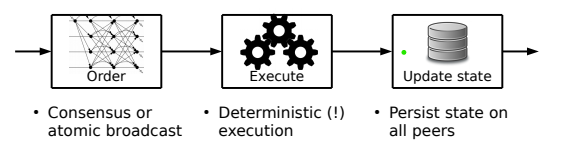
\includegraphics[scale=0.9]{order-execute}
  \caption{Order-execute architecture in replicated services}
  \source{\cite{androulaki_hyperledger_2018}}
\end{figure}

Whilst the order-execute architecture is conceptually simple and therefore widely used, there are drawbacks which occur when using it for a general-purpose permissioned blockchain.\cite{androulaki_hyperledger_2018}
The most significant disadvantages are as follows: 
\emph{Sequential execution}. Executing transactions sequentially on all peers limits the effective throughput that can be achieved on the blockchain.\cite{androulaki_hyperledger_2018} 
One solution to this problem, used by Ethereum \cite{wood_ethereum_nodate}, utilises the concept of \emph{gas} consumed by a transaction execution, which is converted at a \emph{gas price} to a cost in the cryptocurrency and billed to the transaction submitter.
This solution is excellent for use in permissionless blockchains, though does not suffice when designing a general-purpose, permissioned, token-agnostic, blockchain like Hyperledger Fabric. \cite{androulaki_hyperledger_2018}

Hyperledger Fabric distributed applications consist of two parts: A smart contract, called \emph{chaincode}, which is program code that implements the appllication logic and runs during the \emph{execution phase}.
As well as an \emph{endorsment policy} that is evaluated in the \emph{validation phase}.

\subsection{Architecture Overview}
Hyperledger projects follow a design philosophy, which includes a modular, extinsible approach; enabling interoperability.
Design puts an emphasis on secure solutions, crucial to systems using sensitive data.
Hyperledger's token-agnostic approach simplifies bringing blockchain to business infrastructure. \cite{noauthor_hyperledger_2017}

Hyperledger projects embrace security by design and follow the best practices specified by the Linux Foundation's Core Infrastructure initiative. \url{https://www.coreinfrastructure.org/}

\subsection{Privacy by Design}

\url{https://www.hyperledger.org/blog/2018/10/23/private-data-collections-a-high-level-overview} $<--$ private data collections, is privacy by design - enables GDPR compliancy etc 
\url{https://www.researchgate.net/publication/330748854_The_privacy_protection_mechanism_of_Hyperledger_Fabric_and_its_application_in_supply_chain_finance} $<--$ The privacy protection mechanism of Hyperledger Fabric and its application in supply chain finance
\url{https://www.tcs.com/content/dam/tcs/pdf/discover-tcs/Research-and-Innovation/Privacy-by-Design-Helps-blockchains-comply-With-GDPR.pdf} $<--$ Privacy by Design Helps Blockchains Comply With GDPR

\subsection{Inspiration} %- from hyperledger fabric projects, redo title
Use $-->$ \cite{yuan_design_2018}. <-- says there is a "LACK OF UNIVERSALLY DEFINED STANDARDS" is this true still? should this report be proposing standards for blockchain healthcare systems, are there thusfar?

\subsection{Consensus}
Distributed systems \& consensus, use \cite{lamport_byzantine_1982}. \linebreak[1]

The consensus problem occurs when attempting to achieve reliability in a distributed system, in the presence of faulty processes. 
A system requires processes to reach an \emph agreement on a value after one or more processes propose what the value should be. 
In a system such that: each process $p_i$ communicates with other processes via message passing (assuming communication is reliable), up to some number $f$ of the $N$ processes are faulty, the remainder of processes are correct.\linebreak[1]
Reaching consensus is achieved as follows. 
Every process $ p_i $ starts in an \emph{undecided} state and \emph{proposes} a single value $v_i$.
The processes communicate with eachother and exchange values. 
Each process then sets the value of a \emph{decision variable}, $d_i$. 
In doing so the process enters the \emph{decided} state and can no longer change $d_i$.\cite{coulouris_distributed_2011}
\begin{enumerate}
	\item Termination: Eventually each correct process sets a decision variable.
	\item Agreement: The decision of all correct processes is the same.
	\item Integrity: If the correct processes al proposed the same value, then any correct process in the \emph{decided} state has chosen that value.\cite{coulouris_distributed_2011}
\end{enumerate}

In Hyperledger business blockchain frameworks consensus is reached by performing two seperate activities:
\begin{enumerate}
  \item Ordering of transactions
  \item Validating transactions
\end{enumerate}
In the first step, the transactions are received from the client.
An ordering service is used to order the transactions. 
To enable confidentiality, the ordering service may be agnostic to the transaction; that is, the transaction content can be hashed or encrypted.\cite{noauthor_hyperledger_2017}
This is extremely benificial to this system, as maintaining confidentiality is essential to abiding by the GDPR \cite{noauthor_general_nodate}.

Consensus in Hyperledger Fabric is broken into 3 phases: \emph{Endorsement}, \emph{Ordering} and \emph{Validation}.
\begin{enumerate}
  \item Endorsement is driven by policy (eg. m of n signatures) upon which participants endorse a transaction. 
  \item Ordering phase accepts the endorsed transactions and agrees to the order to be committed to teh ledger.
  \item Validation takes a block of ordered transactions and validates the correctness of the results, including checking endorsement policy and double-spending.
\end{enumerate}
zero-knowledge asset transfer vs zero-knowledge proof? \linebreak[1]
Using Go chaincode, generating UML diagrams from this, classes such as: Record, with states: immunised or not?

\section{System Architecture Overview}

going to call the "admissions staff" (people who want to check immunisation information) 



\section{Chaincode}

\cite{alexaki_blockchain-based_2018} suggests that medical records should contain metadata of a patient-provider encounter (visit date/time, location, etc.), 
the data stored off-chain and should be entered when the record is produced. As immunisations expire, the ledger must store metadata on immunisations to ensure the record in the ledger can be invalidated when the date is reached.

Chaincode is Hyperlegder Fabric's version of smart contracts. Chaincode is a program, which can be written in general-programming languages Go, JavaScript (for Nodejs runtime) or Java, that implements a prescribed interface.

Selected Go, as there are apparent benifits outlined in \cite{foschini_hyperledger_2020}

The duration of protection conferred by vaccines should
be tied to passport expiry dates \cite{dye_covid-19_2021}.
This is implemented via the expiration of our immunisation record contract.

\chapter{Immunisation verification}
smarthealth.cards by Vaccination Credential Initiative (VCI) - smart card framework.\linebreak[1]

Use an SDK to invoke chaincode that compares the provided data (hash of the transaction? - in which your immunisation record is stored) with the hash (SHA-250 probs) of the data in the ledger. If there's no match there's no verification, details?

\chapter{Blockchian-as-a-Service}

Using Blockchain for Electronic Health Records \url{'https://ieeexplore.ieee.org/stamp/stamp.jsp?tp=&arnumber=8863359'} \cite{shahnaz_using_2019} 


**shortcomings are discussed here: \url{'https://ieeexplore.ieee.org/document/9284197'} \cite{brotsis_security_2020} ** . The computing power and security provided by BaaS can make up for the shortcomings aforementioned.\cite{song_research_2021}.

Comparing Blockchain-as-a-Service platforms, to identify which tool is most suitable for delpoying the proposed Distributed Immunisation Information System built with Hyperledger Fabric.\linebreak[1]

Reading \cite{onik_performance_2019}.\linebreak[1]

[Performance Analytical Comparison of Blockchain-as-a-Service (BaaS) Platforms] says "Blockchain highly suffers from scalability problem due to its capped transaction
latency as well as consensus approach"\linebreak[1]

Azure have FHIR API, is it the only one? looks like maybe Amazon also \url{'https://azure.microsoft.com/en-gb/services/azure-api-for-fhir/?ocid=AID754288&wt.mc_id=azfr-c9-scottha%2CCFID0475'}{Azure FHIR API}
\linebreak[1]

Beginning, I was aware of two options: Azure and IBM.\linebreak[1]

\section{IBM Blockchain Platform}
IBM Blockchain Platform for IBM Cloud is built with Hyperledger Fabric v1.4.11 and v2.2.2. The system proposed in this report uses v2.2.2, as it delivers delivers important new features and changes for users and operators alike, including support for new application and privacy patterns, enhanced governance around smart contracts, and new options for operating nodes. \cite{noauthor_whats_nodate}

May have to use IBM just because of their whole hybrid cloud infrastructure, could be too easy to give up \cite{noauthor_ibm_2020}
\linebreak[1]
Requested demo of IBM Health Pass, will look more into this physically when the change occurs. For now, review the literature provided publicly - not much lmao \url{'https://www.ibm.com/watson/health/resources/digital-health-pass-blockchain-explained/'}
\url{'https://mytechdecisions.com/compliance/ibm-salesforce-work-covid-19/'}

\chapter{Conclusion}
This should be an assessment of the finished product.

Have you met your objectives? If not, why not?

Suggestions for future extensions

Alternatives methodologies might lead to a better system

\appendix
\chapter{Appendix Title}
\section{Test network} Used for initial testing of chaincode, available on GitHub \footnote{https://github.com/hyperledger/fabric-samples/tree/main/test-network} \label{appendix:testnet}

\section{Chaincode} 
The chaincode developed for the DIIS, representing immunisation records. \footnote{Adapted from tutorial provided in official documentation for Hyperledger Fabric "https://hyperledger-fabric.readthedocs.io/en/release-2.2/chaincode4ade.html"}
\begin{lstlisting}[language=Go, caption={Chaincode representing immunisation records.}]

package main

import (
  "encoding/json"
  "fmt"
  "log"
  //"time"

  "github.com/hyperledger/fabric-contract-api-go/contractapi"
)

// Record provides functions for managing an Asset
   type Record struct {
      contractapi.Contract
    }

// medical records should contain metadata of a patient-provider encounter (visit date/time, location, etc.), 

// Asset describes basic details of what makes up a simple asset
   type Asset struct {
      ID             string `json:"ID"`
      Timestamp          string `json:"dateTime"`
      Owner          string `json:"owner"`
      Expiration     uint64    `json:"expiration"`
    }

// InitLedger adds a base set of assets to the ledger
   func (s *Record) InitLedger(ctx contractapi.TransactionContextInterface) error {
    assets := []Asset{
      {ID: "asset1", Timestamp: "2012-10-31 15:50:13.793654 +0000 UTC", Owner: "Tomoko", Expiration: 104467440737095516},
      {ID: "asset2", Timestamp: "2011-10-21 12:07:13.793654 +0000 UTC", Owner: "Brad", Expiration: 438579485745748},
      {ID: "asset3", Timestamp: "2009-01-11 13:12:13.263674 +0000 UTC", Owner: "Jin Soo", Expiration: 89273489237483},
      {ID: "asset4", Timestamp: "2020-03-13 11:03:13.795664 +0000 UTC", Owner: "Max", Expiration: 239048203894},
      {ID: "asset5", Timestamp: "2019-11-05 14:12:11.798454 +0000 UTC", Owner: "Adriana", Expiration: 9023423948333},
      {ID: "asset6", Timestamp: "2013-05-21 10:01:13.274683 +0000 UTC", Owner: "Michel", Expiration: 290378489237},
    }

    for _, asset := range assets {
      assetJSON, err := json.Marshal(asset)
      if err != nil {
        return err
      }

      err = ctx.GetStub().PutState(asset.ID, assetJSON)
      if err != nil {
        return fmt.Errorf("failed to put to world state. %v", err)
      }
    }

    return nil
  }

// CreateAsset issues a new asset to the world state with given details.
   func (s *Record) CreateAsset(ctx contractapi.TransactionContextInterface, id string, timestamp string, owner string, expiration uint64) error {
    exists, err := s.AssetExists(ctx, id)
    if err != nil {
      return err
    }
    if exists {
      return fmt.Errorf("the asset %s already exists", id)
    }

    asset := Asset{
      ID: id,
      Timestamp:  timestamp,
      Owner:  owner,
      Expiration: expiration,
    }
    assetJSON, err := json.Marshal(asset)
    if err != nil {
      return err
    }

    return ctx.GetStub().PutState(id, assetJSON)
  }

// ReadAsset returns the asset stored in the world state with given id.
   func (s *Record) ReadAsset(ctx contractapi.TransactionContextInterface, id string) (*Asset, error) {
    assetJSON, err := ctx.GetStub().GetState(id)
    if err != nil {
      return nil, fmt.Errorf("failed to read from world state: %v", err)
    }
    if assetJSON == nil {
      return nil, fmt.Errorf("the asset %s does not exist", id)
    }

    var asset Asset
    err = json.Unmarshal(assetJSON, &asset)
    if err != nil {
      return nil, err
    }

    return &asset, nil
  }

// UpdateAsset updates an existing asset in the world state with provided parameters.
   func (s *Record) UpdateAsset(ctx contractapi.TransactionContextInterface, id string, timestamp string, owner string, expiration uint64) error {
    exists, err := s.AssetExists(ctx, id)
    if err != nil {
      return err
    }
    if !exists {
      return fmt.Errorf("the asset %s does not exist", id)
    }

    // overwriting original asset with new asset
    asset := Asset{
      ID: id,
      Timestamp:  timestamp,
      Owner:  owner,
      Expiration: expiration,
    }
    assetJSON, err := json.Marshal(asset)
    if err != nil {
      return err
    }

    return ctx.GetStub().PutState(id, assetJSON)
  }

  // DeleteAsset deletes an given asset from the world state.
  func (s *Record) DeleteAsset(ctx contractapi.TransactionContextInterface, id string) error {
    exists, err := s.AssetExists(ctx, id)
    if err != nil {
      return err
    }
    if !exists {
      return fmt.Errorf("the asset %s does not exist", id)
    }

    return ctx.GetStub().DelState(id)
  }

// AssetExists returns true when asset with given ID exists in world state
   func (s *Record) AssetExists(ctx contractapi.TransactionContextInterface, id string) (bool, error) {
    assetJSON, err := ctx.GetStub().GetState(id)
    if err != nil {
      return false, fmt.Errorf("failed to read from world state: %v", err)
    }

    return assetJSON != nil, nil
  }

// TransferAsset updates the owner field of asset with given id in world state.
   func (s *Record) TransferAsset(ctx contractapi.TransactionContextInterface, id string, newOwner string) error {
    asset, err := s.ReadAsset(ctx, id)
    if err != nil {
      return err
    }

    asset.Owner = newOwner
    assetJSON, err := json.Marshal(asset)
    if err != nil {
      return err
    }

    return ctx.GetStub().PutState(id, assetJSON)
  }

// GetAllAssets returns all assets found in world state
   func (s *Record) GetAllAssets(ctx contractapi.TransactionContextInterface) ([]*Asset, error) {
// range query with empty string for startKey and endKey does an
// open-ended query of all assets in the chaincode namespace.
    resultsIterator, err := ctx.GetStub().GetStateByRange("", "")
    if err != nil {
      return nil, err
    }
    defer resultsIterator.Close()

    var assets []*Asset
    for resultsIterator.HasNext() {
      queryResponse, err := resultsIterator.Next()
      if err != nil {
        return nil, err
      }

      var asset Asset
      err = json.Unmarshal(queryResponse.Value, &asset)
      if err != nil {
        return nil, err
      }
      assets = append(assets, &asset)
    }

    return assets, nil
  }

  func main() {
    assetChaincode, err := contractapi.NewChaincode(&Record{})
    if err != nil {
      log.Panicf("Error creating record chaincode: %v", err)
    }

    if err := assetChaincode.Start(); err != nil {
      log.Panicf("Error starting record chaincode: %v", err)
    }
  }
\end{lstlisting}
\label{appendix:chaincode}


\end{flushleft}

\printbibliography

\end{document}
